\section{Parte 04 – Instalacion de Oracle Data 12C} 

\begin{enumerate}[1.]
	\item Como primer paso para la instalaci\'on del Windows Server 2012 descargamos los iso y el archivo de instalaci\'on\\
	\begin{center}
	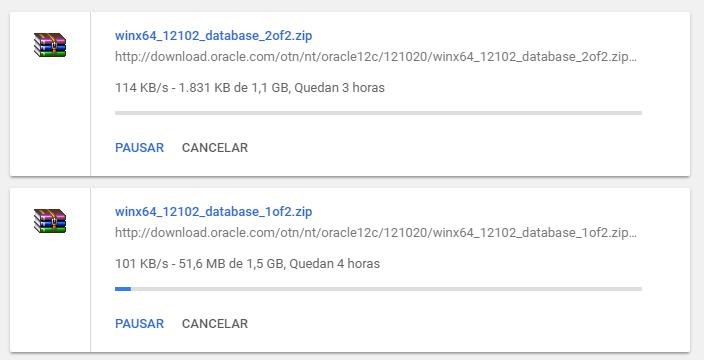
\includegraphics[width=15cm]{./Imagenes/img1} 
	\end{center}

	\item Luego ingresamos al panel de control de administrador de Windows Server\\
	\begin{center}
	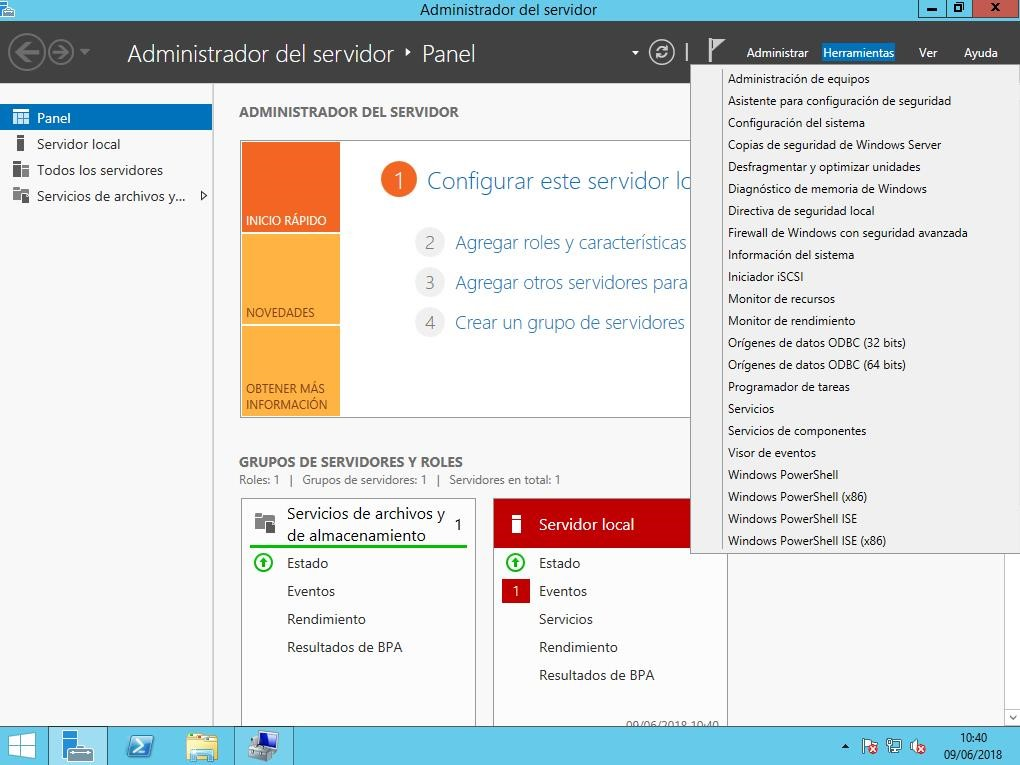
\includegraphics[width=15cm]{./Imagenes/img2} 
	\end{center}


	\item Ingresamos a la Opci\'on Administraci\'on de equipos y presionamos el bot\'on de Deshabilitada\\
	\begin{center}
	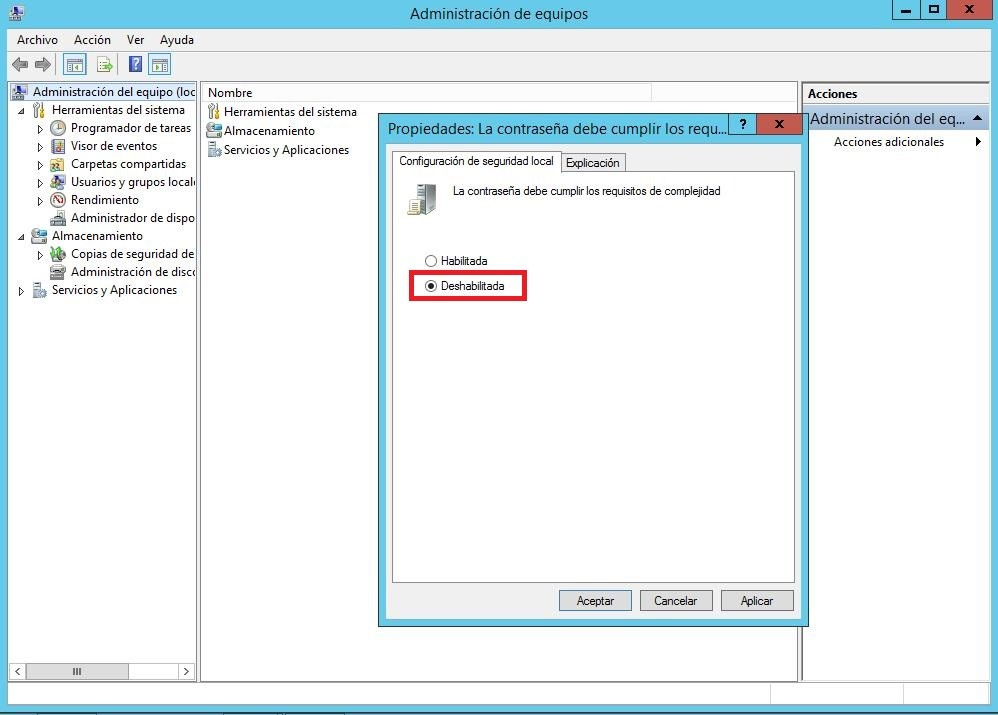
\includegraphics[width=15cm]{./Imagenes/img3} 
	\end{center}

	\item Regresamos al administrador de servicio y presionamos la opci\'on de herramientas\\
	\begin{center}
	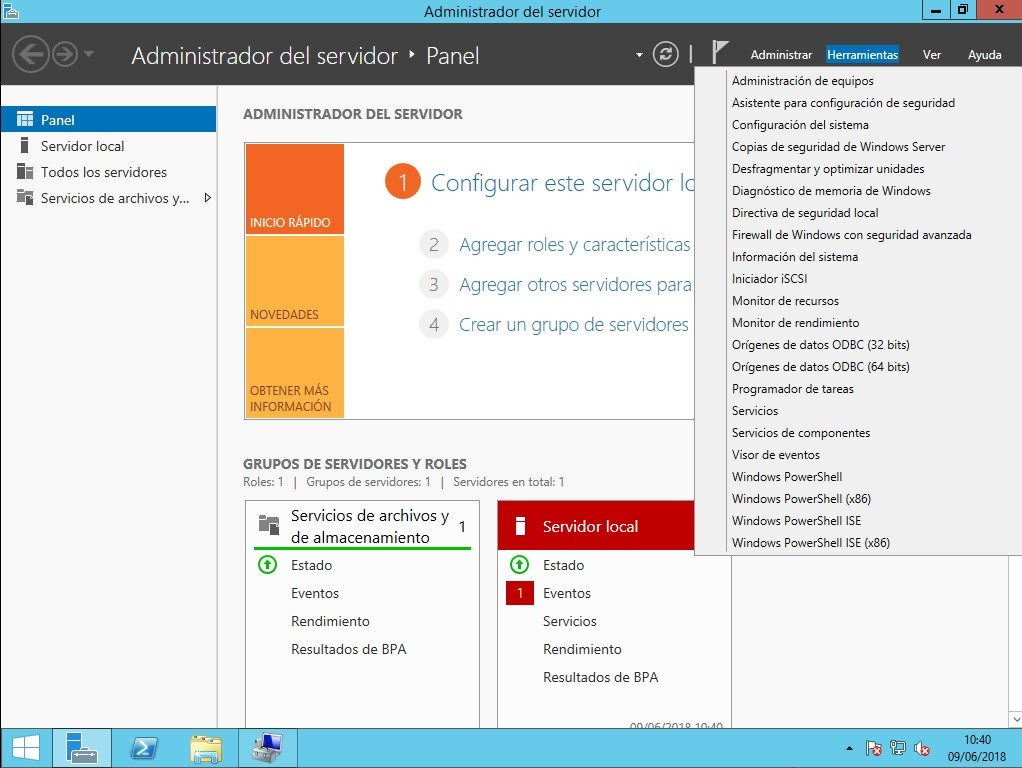
\includegraphics[width=15cm]{./Imagenes/img4} 
	\end{center}

	\item Ingresamos nuevamente Administraci\'on de equipos y nos vamos a la opci\'on de usuarios y grupos locales\\
	\begin{center}
	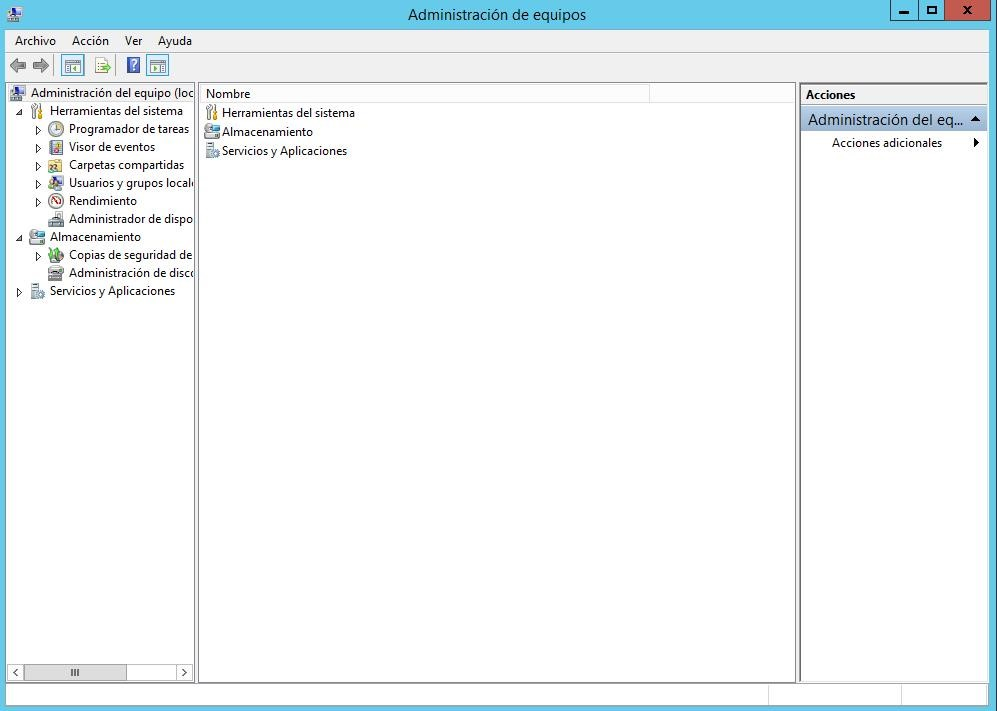
\includegraphics[width=15cm]{./Imagenes/img5} 
	\end{center}

	\item Ingresamos a la carpeta de Usuarios y nos vamos a la opci\'on de equipos ORACLE\\
	\begin{center}
	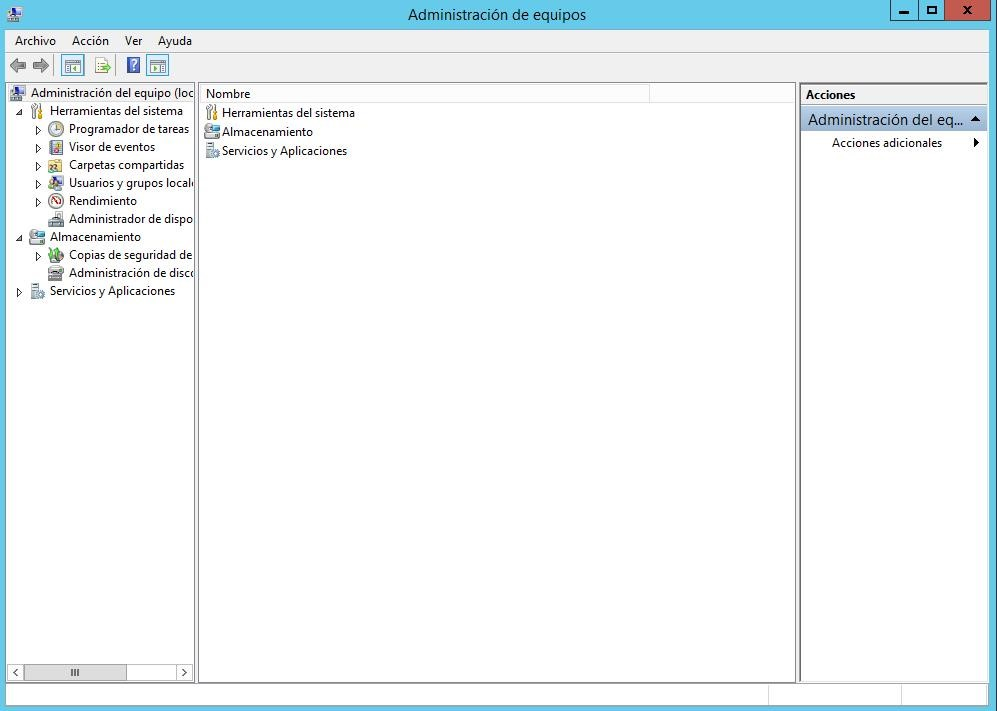
\includegraphics[width=15cm]{./Imagenes/img6} 
	\end{center}

	\item Una vez realizado eso reiniciamos el servidor y al usuario ORACLE \\
	\begin{center}
	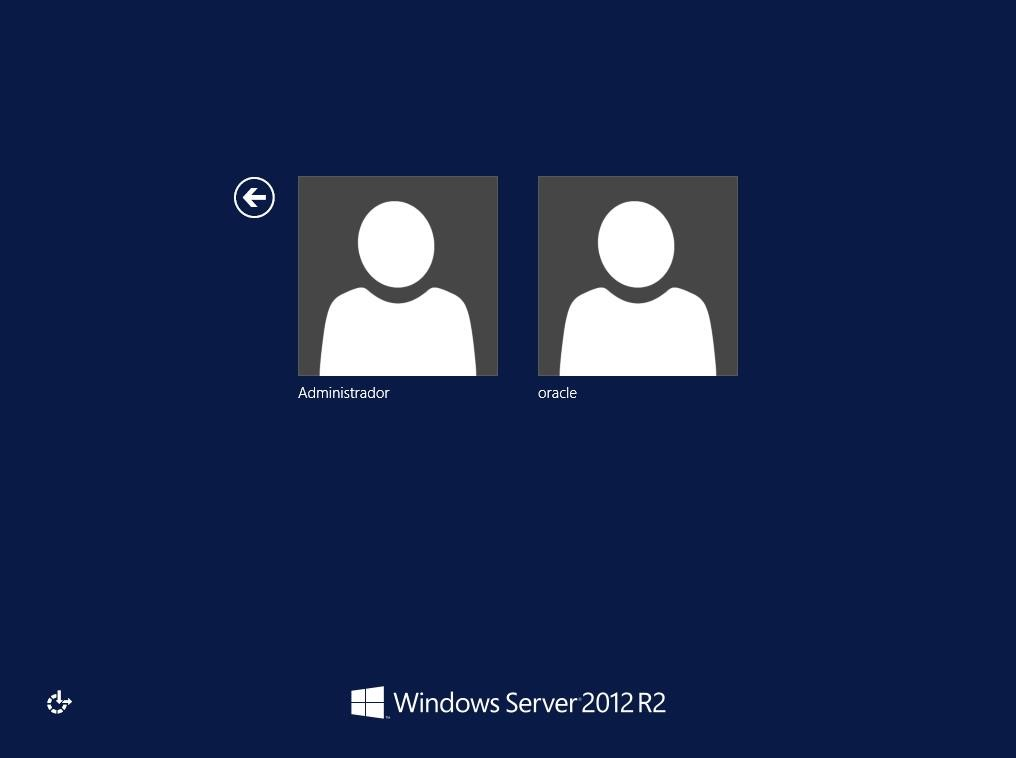
\includegraphics[width=15cm]{./Imagenes/img7} 
	\end{center}

	\item Luego colocamos la clave de administrador UPT2018\\
	\begin{center}
	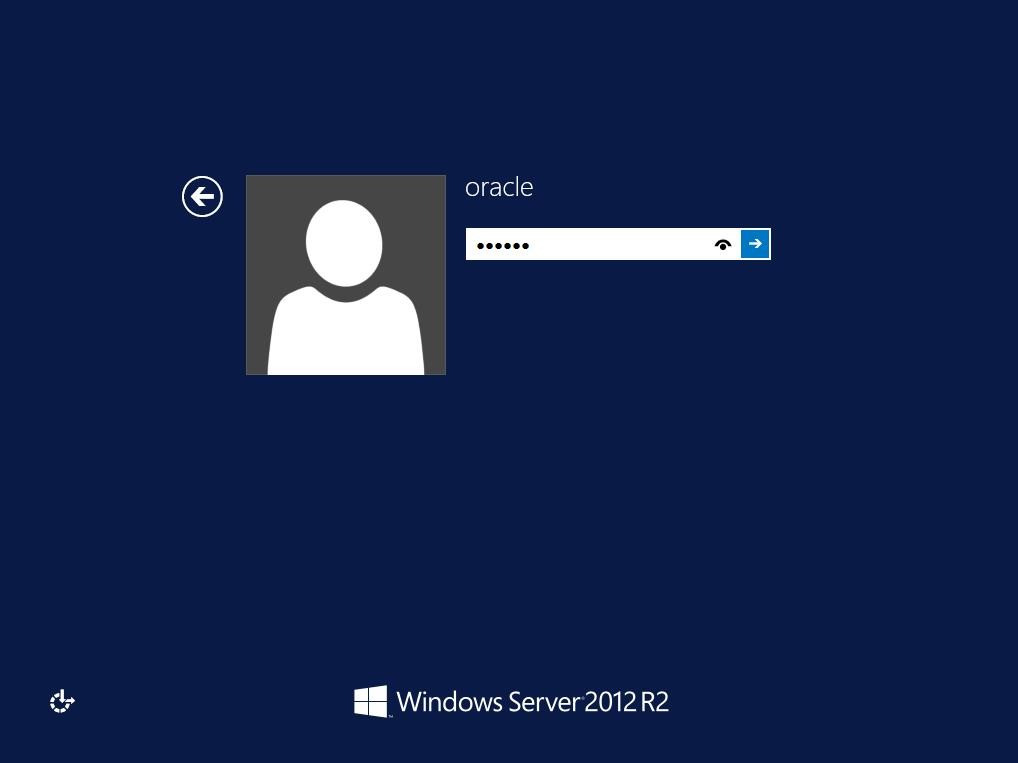
\includegraphics[width=15cm]{./Imagenes/img8} 
	\end{center}

	\item Empezaremos la instalaci\'on de la base de datos ORACLE ingresando a setup\\
	\begin{center}
	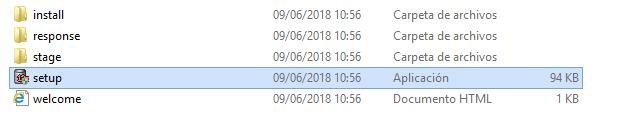
\includegraphics[width=15cm]{./Imagenes/img9} 
	\end{center}

	\item Instalamos en modo de administrador, colocando la clave de usuario\\
	\begin{center}
	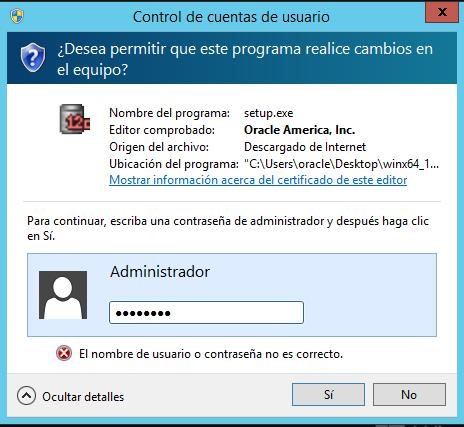
\includegraphics[width=15cm]{./Imagenes/img10} 
	\end{center}

	\item Procede autom\'aticamente la instalaci\'on del ORACLE\\
	\begin{center}
	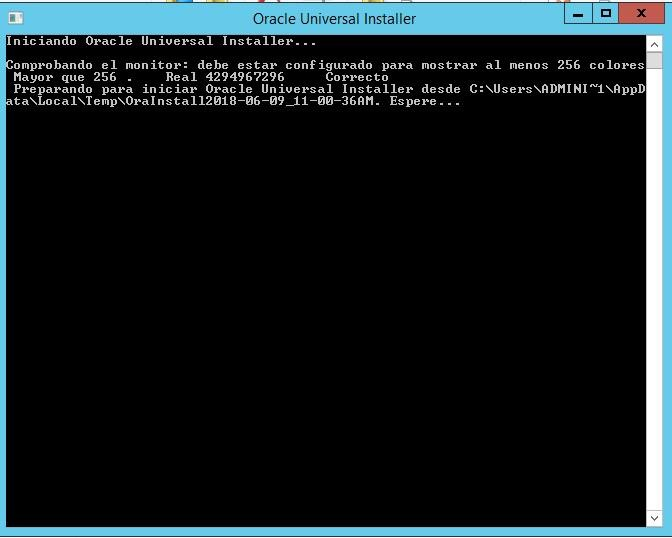
\includegraphics[width=15cm]{./Imagenes/img11} 
	\end{center}

	\item Nos aparece la pantalla de configuraci\'on \\
	\begin{center}
	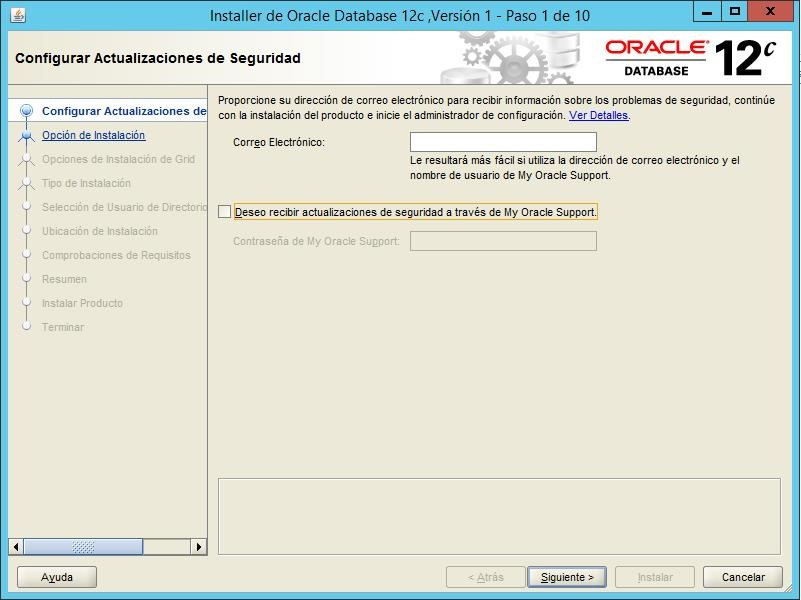
\includegraphics[width=15cm]{./Imagenes/img12} 
	\end{center}

	\item Nos saldr\'a un aviso ingresar su correo electr\'onico, colocaremos si.\\
	\begin{center}
	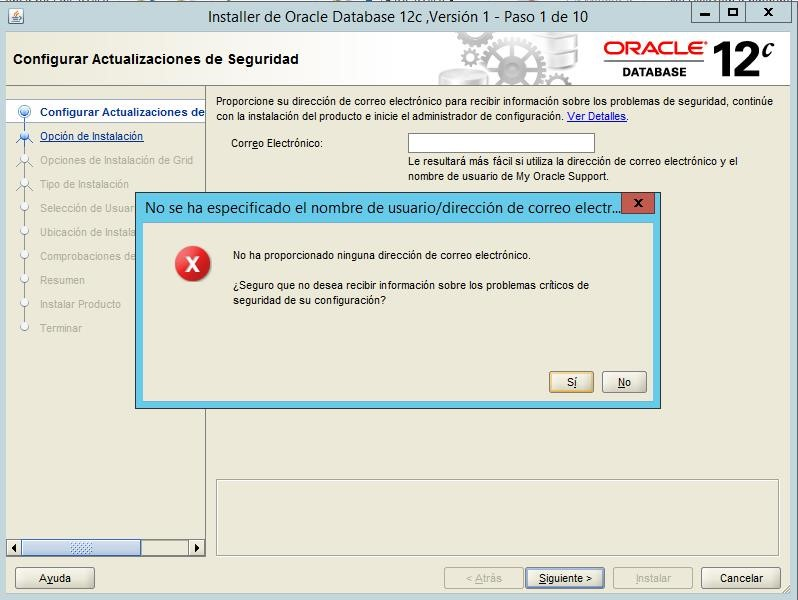
\includegraphics[width=15cm]{./Imagenes/img13} 
	\end{center}

	\item Elegimos la opci\'on de Crear y configurar Base de Datos\\
	\begin{center}
	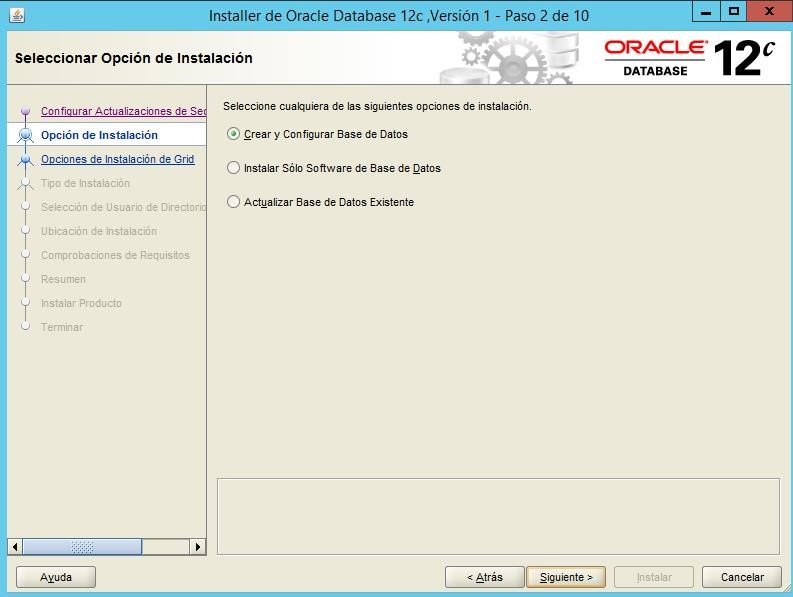
\includegraphics[width=15cm]{./Imagenes/img14} 
	\end{center}

	\item Nos aparecer\'a 2 opciones, que clase de sistema queremos instalar escogemos la opci\'on Clase escritorio\\
	\begin{center}
	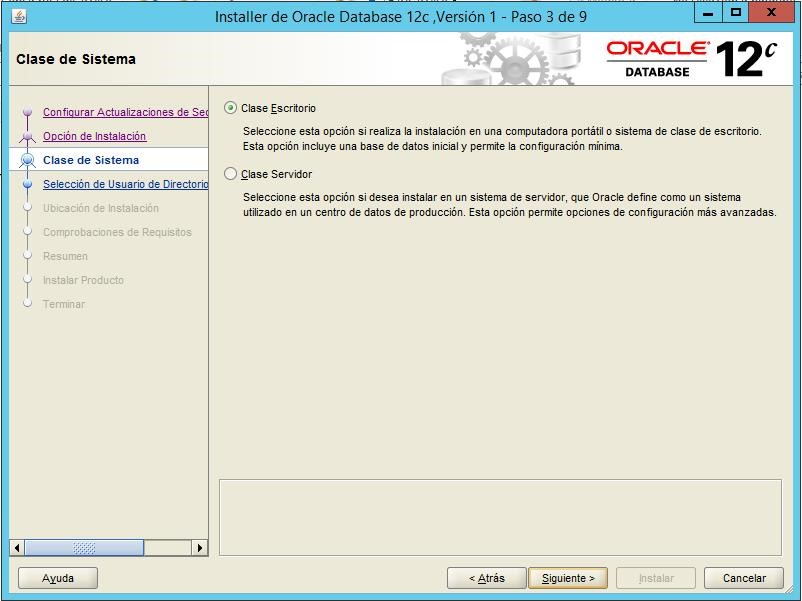
\includegraphics[width=15cm]{./Imagenes/img15} 
	\end{center}

	\item Luego ingresamos con nuestro usuario y contraseña, seleccionamos siguiente\\
	\begin{center}
	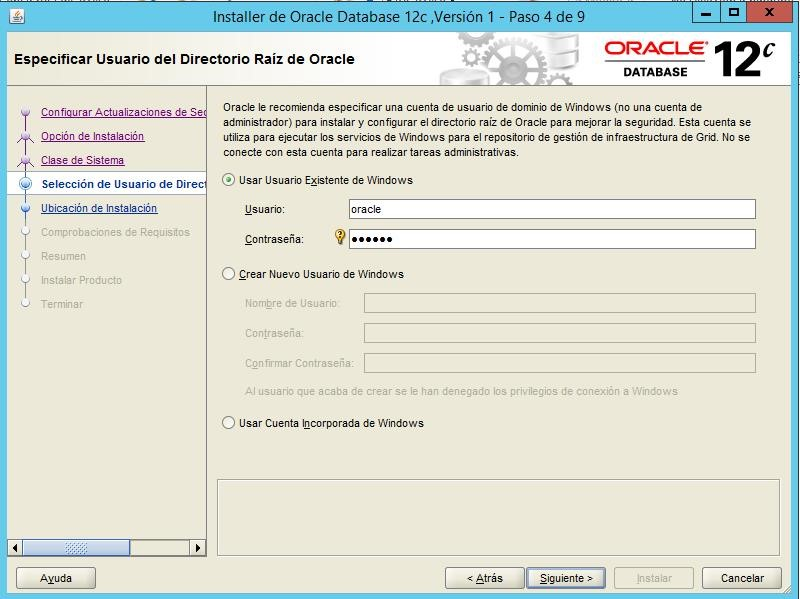
\includegraphics[width=15cm]{./Imagenes/img16} 
	\end{center}

	\item Realizamos las opciones de configuraci\'on, llenando los datos espec\'ificos\\
	\begin{center}
	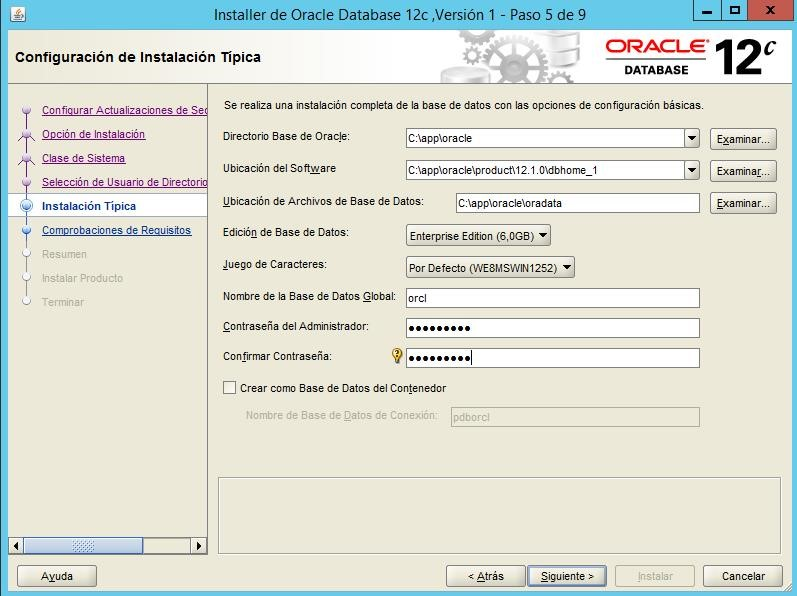
\includegraphics[width=15cm]{./Imagenes/img17} 
	\end{center}

	\item Verificaci\'on de datos y comprobaciones\\
	\begin{center}
	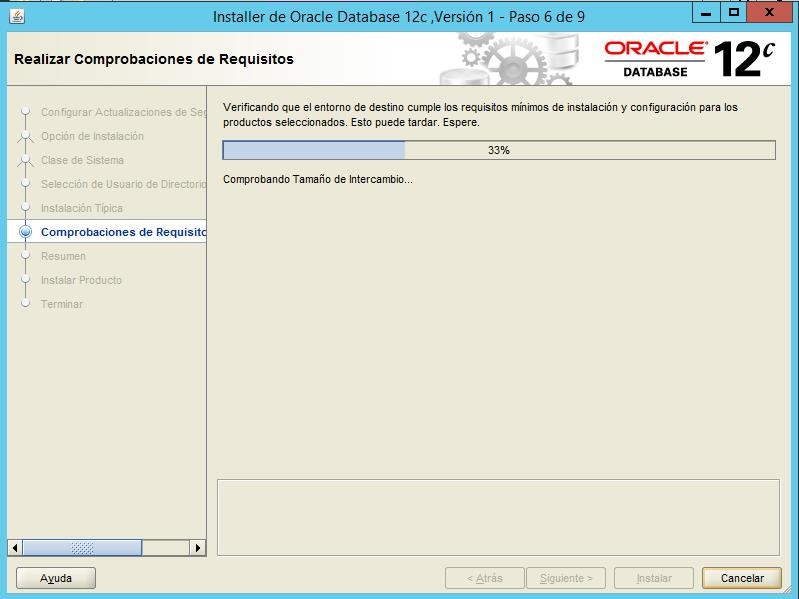
\includegraphics[width=15cm]{./Imagenes/img18} 
	\end{center}

	\item Luego nos muestra una pantalla con el Resumen de instalaci\'on\\
	\begin{center}
	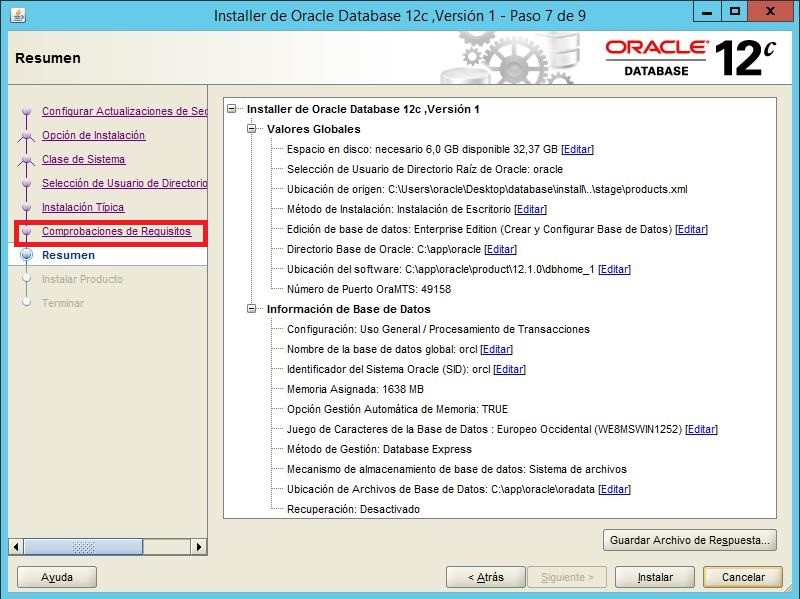
\includegraphics[width=15cm]{./Imagenes/img19} 
	\end{center}

	\item Seguidamente muestra una pantalla de comprobaci\'on nuestros requisitos y colocamos siguientes\\
	\begin{center}
	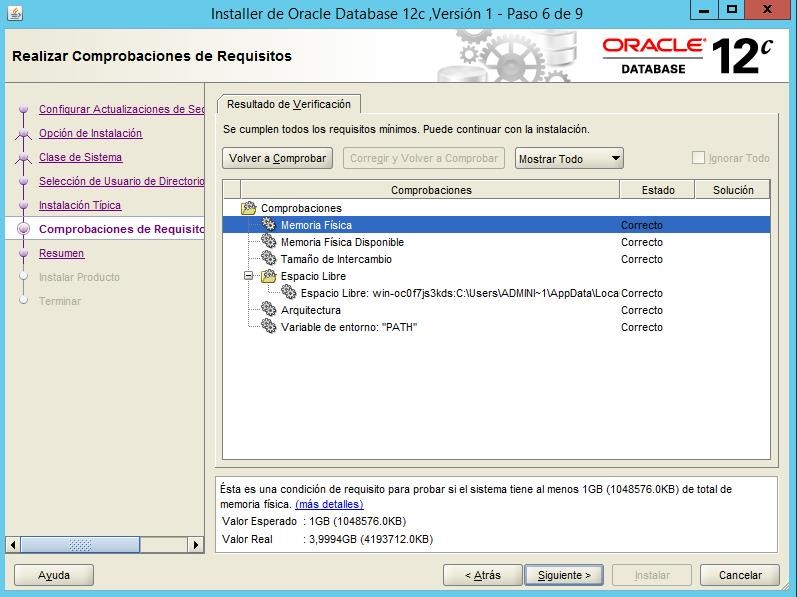
\includegraphics[width=15cm]{./Imagenes/img20} 
	\end{center}

	\item Ingresamos la opci\'on de Instalar\\
	\begin{center}
	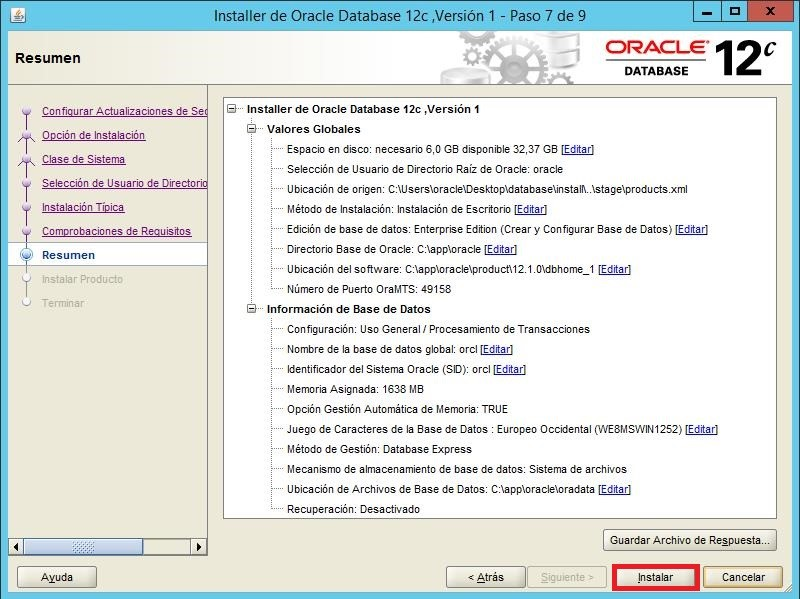
\includegraphics[width=15cm]{./Imagenes/img21} 
	\end{center}

	\item Luego esperemos la instalaci\'on de nuestro programa\\
	\begin{center}
	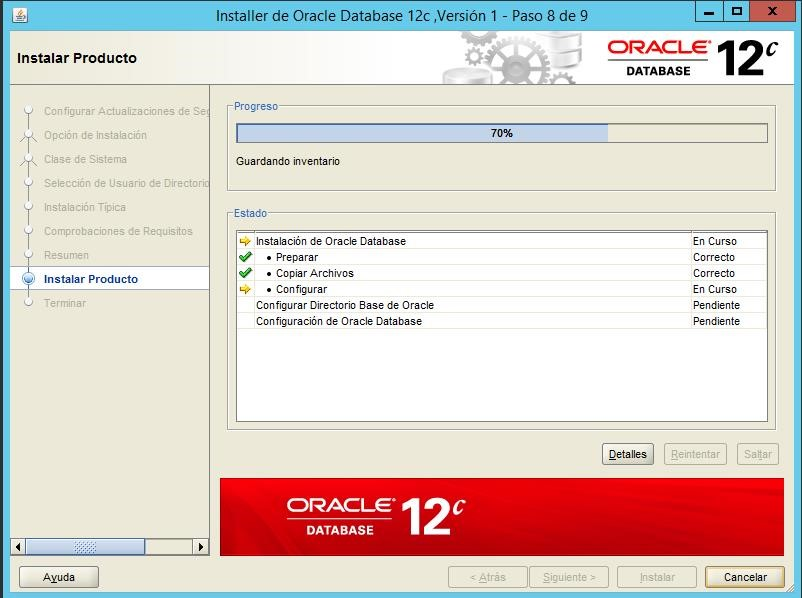
\includegraphics[width=15cm]{./Imagenes/img22} 
	\end{center}

	\item Una vez terminado colocaremos Aceptar\\
	\begin{center}
	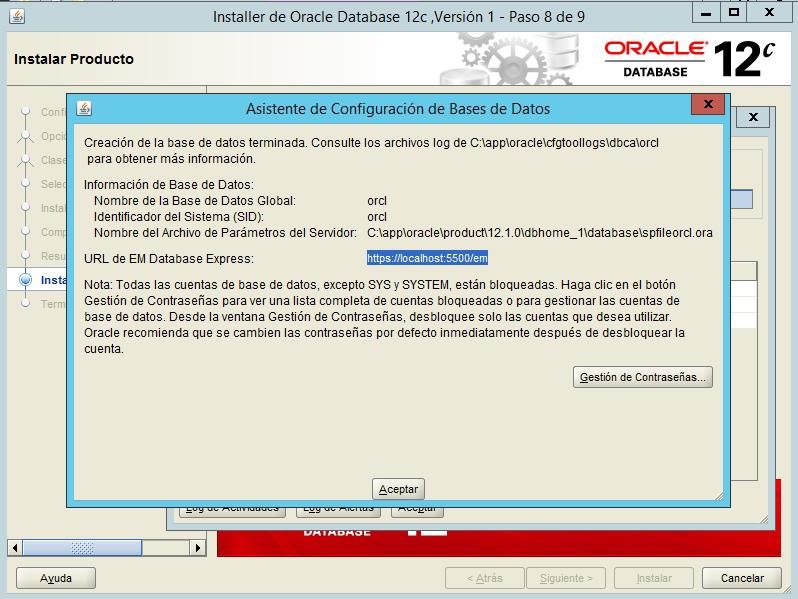
\includegraphics[width=15cm]{./Imagenes/img23} 
	\end{center}

	\item Buscamos el programa SQL DEVELOPER, seguidamente ingresamos a nuestro programa\\
	\begin{center}
	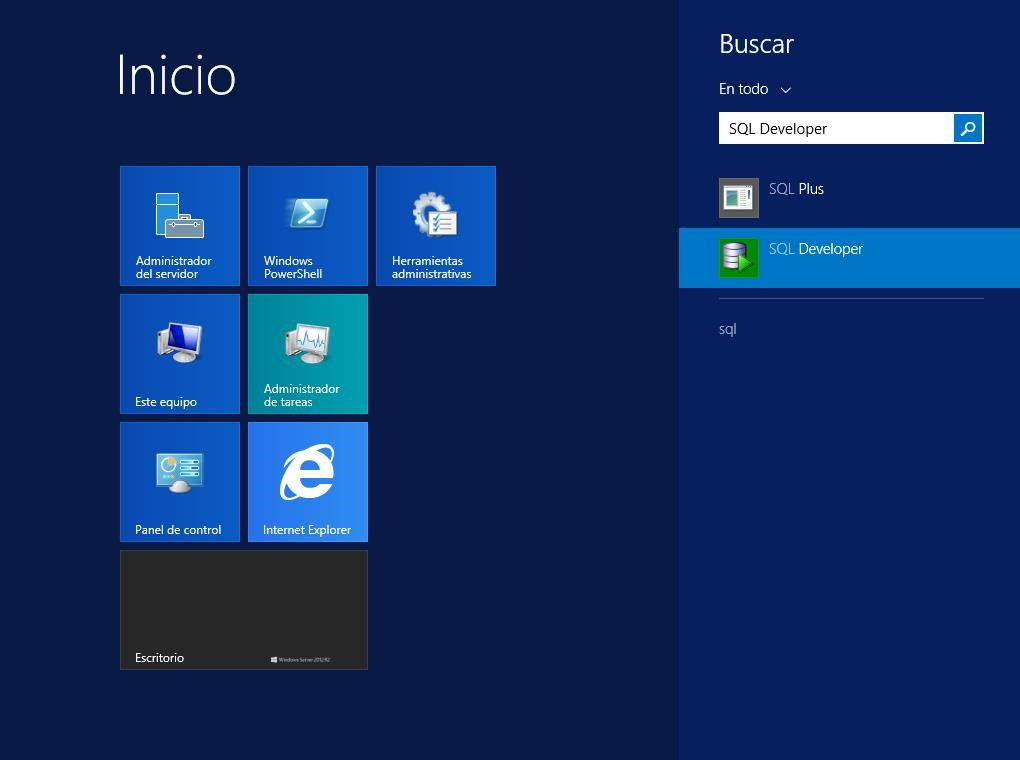
\includegraphics[width=15cm]{./Imagenes/img24} 
	\end{center}

	\item Nos saldr\'a un cuadro donde nos pedir\'a que ingresemos nuestra clave de administrador\\
	\begin{center}
	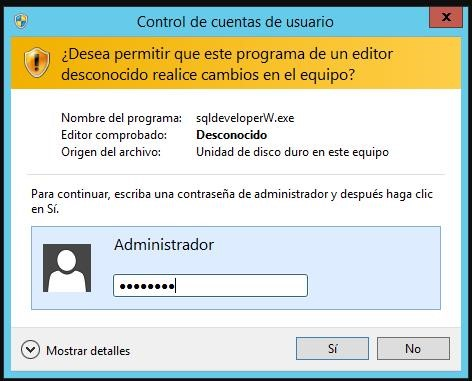
\includegraphics[width=15cm]{./Imagenes/img25} 
	\end{center}

	\item Ingresamos a la opci\'on de Nueva conexi\'on\\
	\begin{center}
	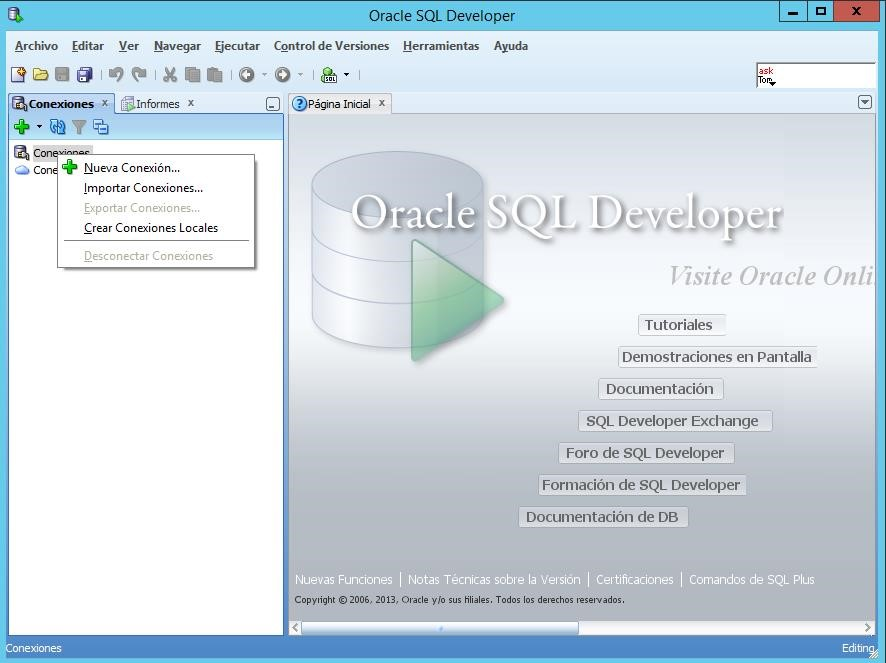
\includegraphics[width=15cm]{./Imagenes/img26} 
	\end{center}

	\item Crearemos nuestra nueva conexi\'on de datos, ingresando todos los datos correspondientes, una vez echo eso colocaremos probar\\
	\begin{center}
	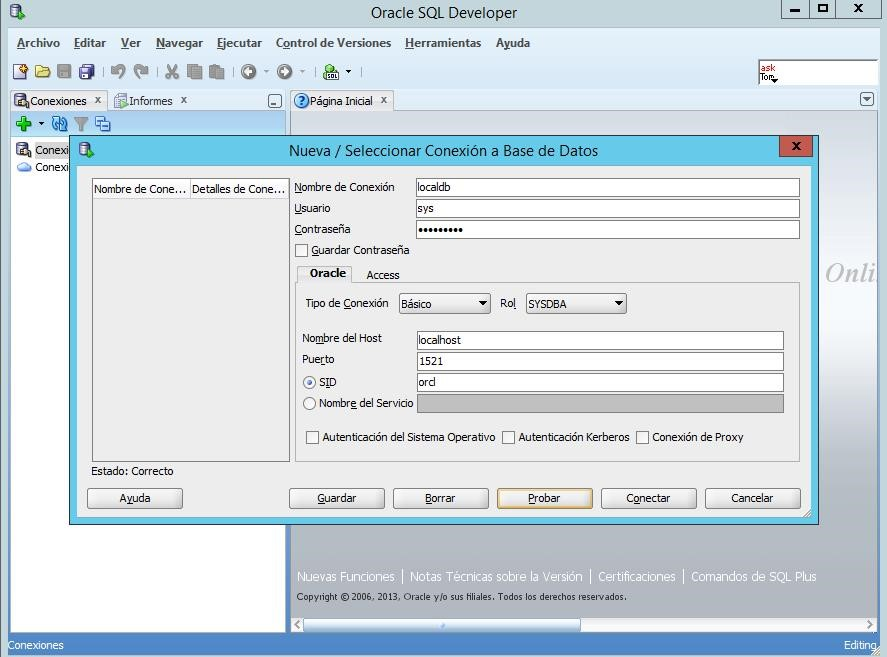
\includegraphics[width=15cm]{./Imagenes/img27} 
	\end{center}

	\item Luego observamos nuestra base de datos creada y lista para su funcionamiento\\
	\begin{center}
	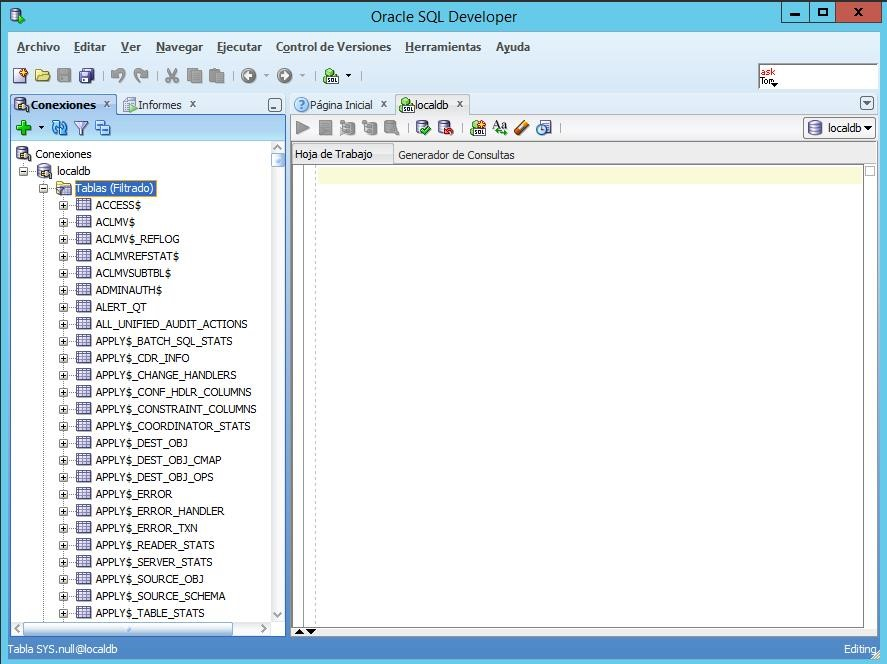
\includegraphics[width=15cm]{./Imagenes/img28} 
	\end{center}


\end{enumerate} 
